\documentclass[11pt]{jarticle}
\usepackage[a4paper, margin=20mm]{geometry}
\usepackage{wrapfig}
\usepackage{jtygm}
\usepackage[dvipdfmx]{graphicx}

\newcommand\gamename{サムライジョッキー}

\title{SamurAI Coding 2017-2018 コンテストルール}
\author{情報処理学会プログラミングコンテスト委員会}
\date{2017/09/16}

\begin{document}
\maketitle

\begin{abstract}
  SamurAI Coding 2017--2018 コンテストの進め方のルールを定める。
  このルール案は暫定版であり, 詳細については今後の改訂の可能性がある.
\end{abstract}

\section{コンテストの概要}
コンテストはネットワーク上で行う予選と、
情報処理学会第80回全国大会に併設して実施する本戦からなる。

\section{参加登録}

\section{予選の構成}
予選は総当りトーナメントの実施が可能な参加チーム数以内ならば、すべての
参加チームが他のすべての参加チームと1ゲーム (スタート位置を交換した2レー
ス) ずつを競う総当り線によって行う。

参加チーム数が多く単純な総当り戦が実施困難である場合は、2次からなる予
選を行う。

1次予選では、参加チームをランダムにいくつかのグループに振り分け、各グ
ループで総当り戦を実施する。1次予選により各グループ上位者を30チーム程
度選抜し、総当り戦での最終予選を行う。

実施に要する手間を軽減するために1次予選の各グループのチーム数は30チー
ム程度に抑える必要がある。このため、参加チームが多ければグループ数を多
くすることで調整する。

1次予選の各グループのチーム数はできる限り均一にする。また、各グループ
から最終予選に進出するチームは同一とする。

\begin{table}
\begin{center}
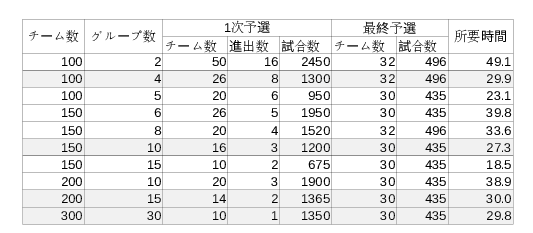
\includegraphics[width=0.8\columnwidth]{preliminary.png}
\caption{参加チーム数に応じた予選の構成例}
\end{center}
\end{table}

\section{総当り戦の方法}
$n$チームによる総当り戦は、毎回対戦相手を変えた$n-1$ステージにより行う。
チーム数が奇数である場合は、主催者がダミーのチームを用意して偶数にして、
すべてのチームがすべてのステージで異なる相手と1ゲームを行うようにする。

ステージごとには異なるコースを用い、
各ステージの全ゲームは同一のコースを用いて行う。
1ゲームは同じコースで出発位置を入れ替えた2レースを行う。
したがって、すべての参加チームは$n-1$種のコースを用いたゲームを各1回、
全部で$2n-2$レースを行うことになる。

総当り戦の順位は、以下の項目をこの順序の優先順位で適用し、最大の者を上位とする。
\begin{enumerate}
\item
  合計勝点。
  各ステージにおいて、ゲームの勝者に2点、敗者に0点、引分の場合には両者に1点を与え、
  全ステージの勝点を合計したもの。
\item
  合計タイム。
  全ステージの全ゲームの両レースについて、ゴールタイムを合計したもの。
  ゴールタイムはゲームルールに定義するものである。
\end{enumerate}

\section{決勝進出チームの決定}
予選上位 (予選を2次に分けて行う場合は、最終予選上位) の12チーム以上を
決勝進出チームとして選抜する。

これに加え、地域などの多様性と予選の戦績を考慮して、最大4チームを決勝
進出チームとして選抜する。

\begin{flushright}
以上
\end{flushright}

\end{document}
